\linespread{1.5}

\textbf{Solução}

\textbf{a)}
\begin{figure}[H]
    \centering
    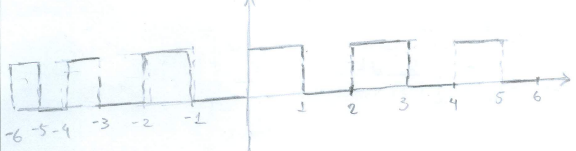
\includegraphics[width=0.7\linewidth]{fig/tl4.png}
\end{figure}

\textbf{b)}
Utilizando a propriedade de atraso de originais, temos:
\begin{equation*}
    f(t) \xrightarrow{\mathcal{L}} F(s) = \frac{G(s)}{1-e^{-Ts}}
\end{equation*}
onde $T$ é o período da função e G(s) é a imagem de $g(t) = h(t) - h(t-1)$

\begin{equation*}
    h(t) - h(t-1) \xrightarrow{\mathcal{L}} \frac{1-e^{-s}}{s}
\end{equation*}

\begin{equation*}
    \boxed{F(s) = \frac{1-e^{-s}}{s(1-e^{-2s})}}
\end{equation*}